%----------------------------------------------------------------------------
\chapter{\bevezetes}
%----------------------------------------------------------------------------

\section{A feladatkiírás részletezése}
A témám alapja egy valós problémára megoldás keresése és annak implementálása. Egy komplett webalkalmazás üzembe helyezése a feladatom, egyedül a kész program forráskódja áll rendelkezésemre, se több, se kevesebb. A cél a weboldal kiszolgálása, annak leállásmentes frissítése, terhelésfüggő skálázása és a kódon dolgozó fejlesztők támogatása.

Bár ez csupán egy példa alkalmazás, minden szempontból megfelel egy valós weboldal igényeinek. A felhasználó elé a frontend oldal kerül mely Reactban\footnote{JavaScript alapú Web keretrendszer - \url{https://reactjs.org/}} íródott. Itt meg lehet tekinteni a megvásárolható termékeket, kategóránkénti bontásban. Ezeket természetesen kosárba lehet helyezni és később megvásárolni azokat. Az alkalmazás chat funkcionalitással is rendelkezik: az oldalt megtekintő felhasználók valós időben küldhetnek egymásnak üzeneteket. A fentebb említett lehetőségeket egy Spring\footnote{Java alkalmazás keretrendszer - \url{https://spring.io/}} használatával írt backend biztosítja, mely gyakorlatilag egy API\footnote{Alkalmazásprogramozási interfész} réteget nyújt a frontend és az adatbázis között. Lehetőséget ad lekérni a kategóriákat, a termékeket, illetve a rendelést leadni (mely adatbázisban \textit{nem} tárolódik). Az adatok PostgreSQL\footnote{Nyílt forráskódú adatbázisszoftver - \url{https://www.postgresql.org/}} adatbázisban tárolódnak.

\textbf{Az feladatom akkor tekinthető sikeresnek, ha az alkalmazás elérhető a felhasználók számára, leállás nélkül lehet frissíteni azt, illetve terheléstől függően skálázódik.}
\subsection{CI/CD}
Első lépésként a fejlesztőkre kell fektetni a hangsúlyt, hogy a szoftver olyan módon legyen tárolva, hogy azt akár többen, egyszerre tudják szerkeszteni anélkül hogy a kódbázis inkonzisztenssé válna. Erre természetesen léteznek megoldások: talán mindenki számára ismert a Git verziókezelő rendszer. De ez még önmagában nem old meg mindent.
\subsubsection{Continuous Integration}
Képzeljük el a következő szituációt: Aladár elkezd dolgozni a projekten, letölti számítógépére a legfrissebb forráskódot Git segítségével. Mivel nem akar problémát abból, hogy többen is ugyanazon kódon dolgoznak így egy külön ágat (branchet) csinál és azon dolgozik.

De mik is azok a branchek? Minden verziókezelt programkódnak van egy \textit{fő ága} amit új verzió kiadásakor alapul veszünk. Ettől szeretnénk leágazni, hogy a saját munkákat úgy tudjuk végezni, hogy közben nem helyezünk el félkész kódot a főágon.\cite{Branch_Git} Ha így tennénk, akkor a következő fejlesztő aki letölti a kódot az eleve sem fogja tudni lefordítani azt (bizonyos esetben).

Aladár képzett programozó, és alapos is: teszteli az alkalmazást mielőtt azt a főágba olvasztaná. Igazából ezzel rengeteg problémát meg is oldottunk, azonban két dolgot nem vettünk figyelembe: az emberi hanyagságot (elképzelhető, hogy Zoltán nem ilyen szorgos és hibás kódot helyez el a főágon), illetve egy speciális esetet: Béla is feladatot kapott, neki is látott egy harmadik ágon a munkának. Dolga végeztél lefutatta a teszteket és látván a hibátlan kimenetet a főágba olvaszotta azt. Aladár is végzett, a lokális tesztek sikeresek, ő is feltölti a kódját és beolvasztja azt. \textit{Az alkalmazás elromlott.} Mi történt?
Aladár fejlesztése függött olyan funkciótól amit időközben Béla szerkeszett és megváltoztatta annak viselkedését. Így hiába működött helyi kódbázison tesztelve, a főág már Béla módosításait is tartalmazta.

\begin{figure}[ht]
\centering
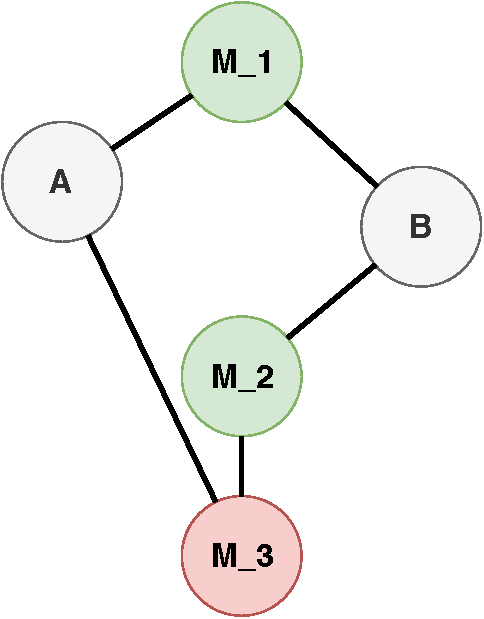
\includegraphics[width=40mm, keepaspectratio]{img/branch_conflict.pdf}
\caption{A fenti példa illusztrálva. Megfigyelhető miként hibásodik meg az alkalmazás.}
\end{figure}

Egy olyan megoldásra lenne szükségünk ami teszteli a főágon megjelenő kódot még mielőtt az ténylegesen odakerülne. Ezt nevezik \textit{Continuous Integration}nak: A CI rendszer automatikusan ellenőrzi a főágba kerülő kódot még az integráció tényleges megtörténte előtt.\cite{CI_Atlassian} Így elértük azt, hogy mindig egy olyan kódbázis álljon a fejlesztők rendelkezésére mely bizonyítottan működőképes. De ez még nem jelenti azt, hogy a felhasználók által aktuális használt verziónak megfelelő kódot fogják szerkeszteni. Ha megbízunk a tesztekben amiket alkalmazásunkhoz írunk, akkor használhatjuk a CI/CD másik felét, a \textit{Continuous Deploymentet}.
\subsubsection{Continuous Deployment}
Continuous Deployment alatt azt értjük, hogy emberi beavatkozás nélkül, automatikusan a felhasználók elé kerül a kész termék. Ennek egyik legnagyobb előnye, hogy a fejlesztők szinte mindig azt a kódbázist kapják melyből a felhasználó előtt szereplő program épült.\cite{CD_Atlassian}

Érdemes megemlíteni, hogy stratégiai döntés lehet az is, hogy nem kerül automatikusan a felhasználók elé a termék, ahhoz emberi beavatkozás kell. Ezt \textit{Continuous Delivery}nek nevezik. Itt gyakorlatilag egy bármelyik pillanatban "élesíthető", lefordított alkalmazás keletkezik, melynek telepítése emberi döntésen múlik.

Létezik köztes megoldás is mely személyes véleményem szerint a legideálisabb. Ha tehetjük akkor tartsunk fent egy - az éles rendszerrel ekvivalens - infrastruktúrát. Itt alkalmazzunk \textit{Continuous Deployment}et, míg az éles rendszeren csak \textit{Continuous Delivery}t: ha a tesztrendszeren valóban működik az alkalmazás, akkor kézzel telepíthetjük azt az éles infrastruktúrára is.
\subsection{Elasztikus skálázás}
Hibamentes alkalmazásunk nagyon megtetszett a felhasználóknak, és szembetaláljuk magunkat azzal a problémával, hogy túlterheltek a szerverek. Mit tehetünk? Több erőforrást adunk a kiszolgálónak, erősebb fizikai gépet, esetleg több példányt indítunk (több szerveren), és egy terheléselosztót illesztünk a program elé. Az elképzelés csodálatos, de van egy apró probléma: nem automatizált, emberi beavatkozás szükséges. Ez egyrészről probléma, mert valószínűleg nem tudjuk időben lekezelni a megnövekedett igényeket, nem tudunk időben felskálázni. Van azonban egy kevésbé nyilvánvaló ok is: költséghatékonyság szempontjából leskáláznunk is fontos, különösen ha felhőszolgáltatót\footnote{Távoli szervereket biztosító szolgáltató} használunk. Az éjjeli órákban egészen biztosan nem fog egy webalkalmazás akkora forgalmat generálni, mint mondjuk egy délután során.

Tehát a skálázás azt jelenti, hogy az alkalamazás számára rendelkezésre álló erőforrások mennyiségét szabályozni tudjuk. De mitől \textit{elasztikus}? Ez jelenti azt, hogy az igények alapján skálázunk. Nagy forgalom esetén fel, alacsony esetén le.\cite{Elastic_Turbonomic}
\section{A probléma fontossága}
A fentiek után azt gondolom nyilvánvaló miért (lenne) fontos minél több cégnek átgondolnia jelenlegi szoftverfejlesztési stratégiáját és élni a modern technológia adta lehetőségekkel. Verziókezelt kódot használni, tesztesetekkel, CI rendszerbe kötve és aztán automatikusan közzétéve, alkalmazástípustól függően skálázva azt.
\section{A tervezett megoldás}
Az eddig leírtak tükrében szeretném a példa webalkalmazás verziókezelését megvalósítani, mégpedig két kiemelt ággal:
\begin{itemize}
    \item \textit{prod} ág: A felhasználó elé kerülő verzió főága.
    \item \textit{beta} ág: Belső fejlesztéshez használt rendszer, teljesen különálló, de a \textit{prod} ággal megegyező infrastruktúrán (értelemszerűen kevesebb erőforrással).
\end{itemize}
Ezeket \textit{Continuous Integration} rendszer fogja védeni. Ide kódot olvasztani csak akkor lehet, ha a tesztek sikeresen lefutottak. Ha ezekre az ágakra új programkód érkezik, akkor ismét tesztelésre kerül, és ha sikerrel jár akkor alkalmazáskép\footnote{Olyan "fájl" mely alapján az alkalmazást el lehet indítani} készül, majd az a megfelelő infrastruktúrán telepítésre is kerül.

Az alkalmazás menedzselését, monitorozását, és a skálázást Kubernetes segítségével tervezem megvalósítani, melyről a továbbiak során szó fog esni.